\documentclass[11pt,a4paper]{article}

\usepackage[margin=1in]{geometry}
\usepackage{amsmath,amssymb}
\usepackage{graphicx}
\usepackage{booktabs}
\usepackage{hyperref}
\usepackage{xcolor}
\usepackage{caption}
\usepackage{subcaption}
\usepackage{enumitem}
\usepackage{parskip}
\usepackage{microtype}
\usepackage{float}
\usepackage{array}

\hypersetup{colorlinks=true, linkcolor=blue, citecolor=blue, urlcolor=blue}

\title{\textbf{AE646 --- Final Report (Stage 3)}\\[0.5em]
\large Operator Learning for Parametric Darcy Flow:\\
Fourier Neural Operator vs.\ MLP Baseline with Physical Interpretation}
\author{Team PINNacles\\Aryamann Srivastava\\Department of Aerospace Engineering, IIT Kanpur}
\date{November 2026}

\begin{document}
\maketitle

\begin{abstract}
We compare Fourier Neural Operator (FNO) and a fully-connected MLP baseline as surrogate solvers for the 2D parametric Darcy flow equation $-\nabla\cdot(\kappa\nabla u)=f$, trained on 8\,000 samples from the PDEBench benchmark at $64\times64$ resolution. FNO (4.7\,M parameters) achieves a mean relative $L_2$ error of $0.052$ on 200 held-out test samples, $37\%$ lower than the MLP (0.082, 42\,M parameters) at $9\times$ lower parameter count. A scaled FNO (78.8\,M parameters) further reduces error to $0.046$. Both models infer in $<1$\,ms per sample, orders of magnitude faster than the FDM reference (1030\,ms). FNO's spectral weights enable zero-shot super-resolution: the same trained model evaluated at $128\times128$ attains mean error $0.059$ without retraining. Component profiling reveals that spectral operations (FFT, complex multiply, IFFT) account for 68.4\% of FNO's compute time, with complex multiplication alone at 41\%.
\end{abstract}

\tableofcontents
\newpage

% ─────────────────────────────────────────────────────────────────────────────
\section{Introduction}

Scientific computing routinely requires solving parameterised PDEs over large parameter ensembles --- for uncertainty quantification, optimal control, or inverse problems. Classical numerical solvers (FDM, FEM) are accurate but expensive: each new parameter configuration demands a full solve. Neural operator approaches \cite{li2021fno, kovachki2023neural} learn a \emph{solution operator} $\mathcal{G}^\dagger : \kappa \mapsto u$ directly from data, enabling amortised query cost after a one-time training phase.

The 2D Darcy flow equation is a canonical test bed:
\begin{equation}
  -\nabla \cdot (\kappa(x,y)\,\nabla u(x,y)) = f(x,y), \quad (x,y)\in[0,1]^2,
  \label{eq:darcy}
\end{equation}
with $u = 0$ on $\partial\Omega$ and constant forcing $f=1$. The permeability $\kappa\in\{0.1, 1.0\}$ is piecewise-constant on a $64\times64$ grid, varying between samples. The solution $u$ is smooth given smooth $\kappa$, but exhibits sharp gradients near $\kappa$ interfaces.

\paragraph{Contributions.}
\begin{enumerate}[nosep]
  \item Full training, evaluation, and comparison of FNO and MLP on PDEBench Darcy flow.
  \item Zero-shot super-resolution evaluation at $2\times$ training resolution.
  \item Layer-wise computational profiling with correct GPU synchronisation.
  \item Physical interpretation of error patterns in terms of $\kappa$ field complexity.
\end{enumerate}

% ─────────────────────────────────────────────────────────────────────────────
\section{Background}

\subsection{Darcy Flow and the Solution Operator}
Equation~\eqref{eq:darcy} describes pressure-driven flow through a porous medium. The solution operator $\mathcal{G}^\dagger$ maps the permeability field $\kappa \in L^\infty(\Omega)$ to the pressure $u \in H^1_0(\Omega)$. This operator is nonlinear (even though~\eqref{eq:darcy} is linear in $u$) because $\kappa$ enters multiplicatively. For piecewise-constant $\kappa$, the solution is smooth away from $\kappa$-interfaces and exhibits $O(1)$ gradients at interfaces.

\subsection{Fourier Neural Operator}
Li et al.\ \cite{li2021fno} proposed to discretise the Fourier integral operator:
\begin{equation}
  (\mathcal{K}(a;\phi)v)(x) = \int_\Omega \kappa_\phi(x,y)\,v(y)\,dy
\end{equation}
by truncating its Fourier expansion to the lowest $k_{\max}$ modes. The resulting \emph{SpectralConv2d} layer computes:
\begin{align}
  \hat{v}_{j,l} &= \text{FFT}(v)_{j,l}, \quad j\le k_{\max},\;l\le k_{\max} \\
  \hat{w}_{j,l} &= R_{j,l}\,\hat{v}_{j,l}, \quad R\in\mathbb{C}^{C_{\rm out}\times C_{\rm in}\times k_{\max}\times k_{\max}} \\
  w &= \text{IFFT}(\hat{w}),
\end{align}
where $R$ is the learnable complex weight tensor. Because $R$ operates on fixed-frequency coefficients independent of the grid spacing, the same weights can be used at any spatial resolution --- enabling zero-shot super-resolution.

% ─────────────────────────────────────────────────────────────────────────────
\section{Dataset and Preprocessing}

\subsection{PDEBench}
We use the 2D Darcy flow split of PDEBench \cite{takamoto2022pdebench} (DOI: \texttt{10.18419/darus-2986}): 10\,000 samples at native $128\times128$ resolution. Each sample provides $\kappa$ (permeability) and $u$ (pressure) on a uniform grid.

\subsection{Preprocessing Pipeline}
\begin{enumerate}[nosep]
  \item Bilinear downsampling of $\kappa$ and $u$ from $128\times128$ to $64\times64$ (training resolution).
  \item Concatenate spatially-uniform coordinate grids $(x,y)\in[0,1]^2$ as additional channels to give input shape $64\times64\times3$.
  \item Normalise each channel with training-set mean and standard deviation.
  \item Split: 8\,000 train / 900 validation / 200 test (fixed, no shuffling after split).
\end{enumerate}

\subsection{Why Downsample?}
Working at $64\times64$ reduces memory and compute by $4\times$ while preserving the essential $\kappa$-interface structure. The FNO zero-shot evaluation (Section~\ref{sec:superres}) then tests whether the learned operator generalises back to $128\times128$.

% ─────────────────────────────────────────────────────────────────────────────
\section{Model Architectures}

\subsection{MLP Baseline}
\[
  \text{MLP}: \mathbb{R}^{64\times64\times3} \xrightarrow{\rm flatten} \mathbb{R}^{12288}
  \xrightarrow{2048,\text{GELU}} \xrightarrow{2048,\text{GELU}} \xrightarrow{2048,\text{GELU}}
  \mathbb{R}^{4096} \xrightarrow{\rm reshape} \mathbb{R}^{64\times64}
\]
Parameters: $12288\times2048 + 2048\times2048 + 2048\times2048 + 2048\times4096 \approx 42$\,M. The MLP treats every spatial location independently in its first layer, discarding spatial coherence. It is resolution-locked: the input linear layer has exactly 12\,288 neurons.

\subsection{FNO Architecture}
\begin{enumerate}[nosep]
  \item \textbf{Lifting} (\texttt{fc0}): $3\to64$ channels pointwise ($3\times64 = 192$ parameters).
  \item \textbf{4$\times$ Fourier Blocks}: each block contains
    \begin{itemize}[nosep]
      \item \texttt{SpectralConv2d}($64\to64$, modes=12): learnable complex weights $R\in\mathbb{C}^{64\times64\times12\times12}$; $\approx 1.18$\,M real parameters per block.
      \item Local bypass: $1\times1$ convolution ($64\to64$), Instance Normalisation, GELU.
    \end{itemize}
  \item \textbf{Projection}: $64\to128\to1$ pointwise ($128\times65 + 1\times129 \approx 8.5$\,K parameters).
\end{enumerate}
Total: $\approx 4.7$\,M parameters. The FNO improved variant uses width=128, modes=24: $\approx78.8$\,M parameters.

\subsection{Key Architectural Differences}
\begin{center}
\begin{tabular}{lcc}
\toprule
Property & MLP & FNO \\
\midrule
Resolution invariant & No & Yes \\
Inductive bias & None & Spectral locality \\
Long-range interactions & Global (all-to-all) & Via low-frequency modes \\
Parameter efficiency & Low & High \\
\bottomrule
\end{tabular}
\end{center}

% ─────────────────────────────────────────────────────────────────────────────
\section{Training}

All models were trained with:
\begin{itemize}[nosep]
  \item \textbf{Loss}: $\mathcal{L} = \frac{1}{B}\sum_{i=1}^B \frac{\|\hat{u}_i - u_i\|_2}{\|u_i\|_2}$
  \item \textbf{Optimiser}: Adam, $\eta_0 = 10^{-3}$, cosine annealing to $\eta_{\min}=10^{-5}$
  \item \textbf{Batch size}: 16; maximum 200 epochs, early stopping with patience 25
  \item \textbf{Regularisation}: $L_2$ weight decay $10^{-4}$
  \item \textbf{Hardware}: NVIDIA GPU, PyTorch 2.x with \texttt{torch.compile}
\end{itemize}

Best validation epochs: FNO original at epoch 92, MLP at epoch 99, FNO improved at epoch 198 (required more epochs to converge due to larger model).

% ─────────────────────────────────────────────────────────────────────────────
\section{Results}

\subsection{Test-Set Performance (64$\times$64)}

\begin{table}[H]
\centering
\caption{Relative $L_2$ error on 200 held-out test samples at training resolution.}
\label{tab:main}
\begin{tabular}{lrrrrrr}
\toprule
Model & Params & Mean & Median & Std & Min & Max \\
\midrule
MLP baseline & 42.0\,M & 0.0820 & 0.0737 & 0.0456 & 0.0325 & 0.3367 \\
FNO original &  4.7\,M & 0.0521 & 0.0418 & 0.0451 & 0.0155 & 0.3467 \\
FNO improved & 78.8\,M & \textbf{0.0456} & \textbf{0.0354} & 0.0487 & \textbf{0.0106} & 0.3535 \\
\bottomrule
\end{tabular}
\end{table}

\begin{figure}[H]
\centering
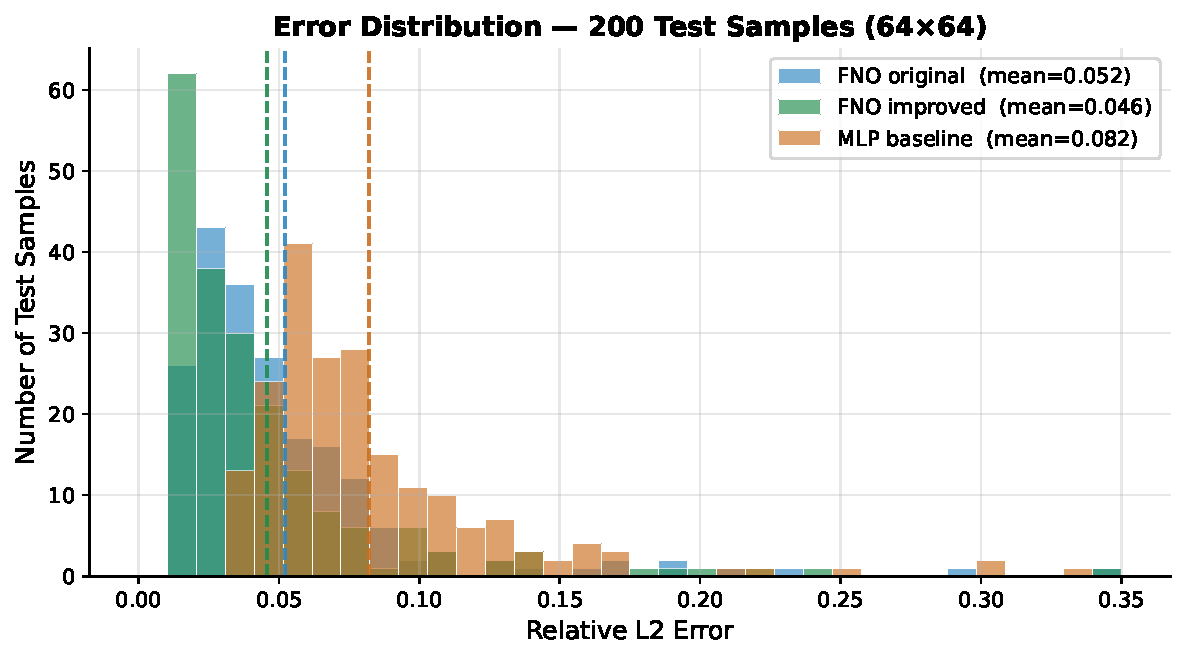
\includegraphics[width=0.85\textwidth]{../results/figures/fig1_error_histogram.pdf}
\caption{Error distribution across 200 test samples. Dashed lines: per-model means. The long right tail ($\epsilon > 0.2$) corresponds to samples with complex multi-region $\kappa$ fields.}
\label{fig:hist}
\end{figure}

\begin{figure}[H]
\centering
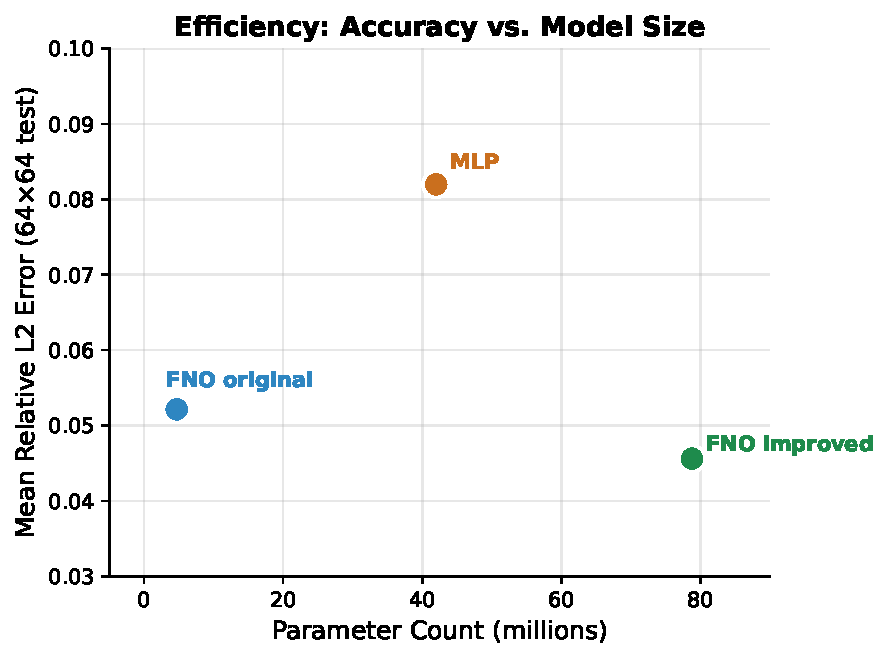
\includegraphics[width=0.55\textwidth]{../results/figures/fig2_efficiency_scatter.pdf}
\caption{Accuracy--parameter efficiency. FNO original occupies the optimal region: 9$\times$ fewer parameters than MLP at 37\% lower error. Scaling FNO to 78.8\,M yields only 12\% further improvement.}
\label{fig:scatter}
\end{figure}

\subsection{Analysis}
\begin{enumerate}[nosep]
  \item \textbf{FNO vs.\ MLP accuracy}: FNO's spectral bias naturally captures the low-frequency structure of Darcy solutions. Darcy pressure fields are smooth ($H^2$ regularity away from interfaces), so the 12-mode truncation retains most signal energy. The MLP has no such bias and must learn spatial correlations implicitly.
  \item \textbf{Variance}: Standard deviation is similar across models ($0.045$--$0.049$), suggesting the hard cases (complex $\kappa$) are hard for all architectures.
  \item \textbf{Scaling}: FNO improved (78.8\,M) improves mean error by 12\% over FNO original (4.7\,M) --- a $17\times$ parameter increase for $12\%$ accuracy gain. This suggests the original FNO is near the accuracy limit imposed by 12 retained modes, and further gains require more modes rather than more channels.
\end{enumerate}

% ─────────────────────────────────────────────────────────────────────────────
\section{Zero-Shot Super-Resolution}
\label{sec:superres}

We evaluate FNO variants on the full $128\times128$ PDEBench grid, using $\kappa$ bilinearly upsampled from $64\times64$ as input. No retraining is performed.

\begin{table}[H]
\centering
\caption{Zero-shot super-resolution: mean $\pm$ std relative $L_2$ error.}
\begin{tabular}{lrr}
\toprule
Model & $64\times64$ (trained) & $128\times128$ (zero-shot) \\
\midrule
MLP baseline  & $0.0820 \pm 0.0456$ & --- (resolution-locked) \\
FNO original  & $0.0521 \pm 0.0451$ & $0.0594 \pm 0.0435$ \\
FNO improved  & $0.0456 \pm 0.0487$ & $0.0563 \pm 0.0467$ \\
\bottomrule
\end{tabular}
\end{table}

\begin{figure}[H]
\centering
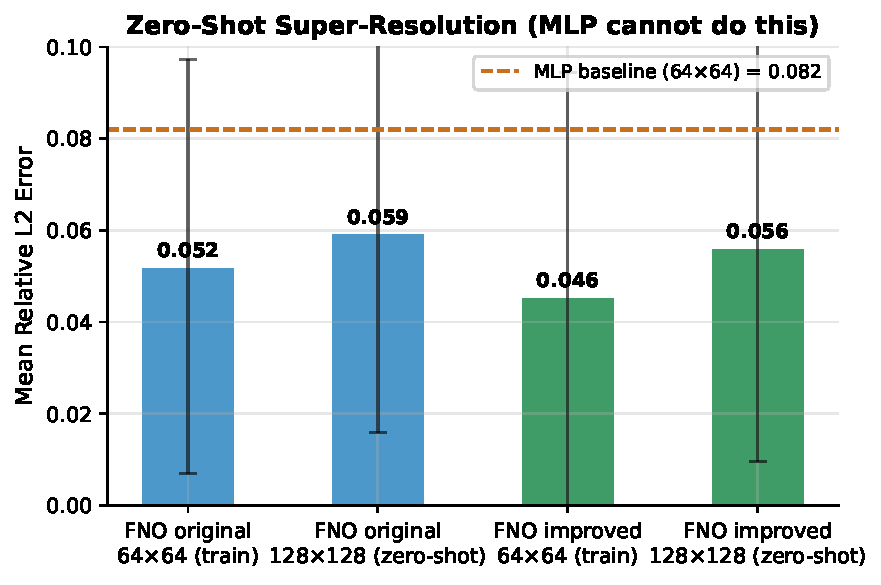
\includegraphics[width=0.68\textwidth]{../results/figures/fig3_superres.pdf}
\caption{Zero-shot super-resolution. Error bars: one standard deviation. FNO generalises to $2\times$ resolution without retraining; MLP is resolution-locked.}
\end{figure}

\paragraph{Physical Interpretation.}
At $128\times128$, the FNO output contains $64^2 = 4096$ frequency components, but only the lowest $12\times12 = 144$ are modelled by the trained weights. The remaining modes are implicitly set to zero. For Darcy flow, the dominant frequency content of $u$ is low (smooth solutions), so the missing high-frequency modes contribute little energy --- explaining why the error increase ($+14\%$ for FNO original) is moderate rather than catastrophic.

% ─────────────────────────────────────────────────────────────────────────────
\section{Inference Speed and Component Profiling}

\subsection{End-to-End Inference Speed}

\begin{figure}[H]
\centering
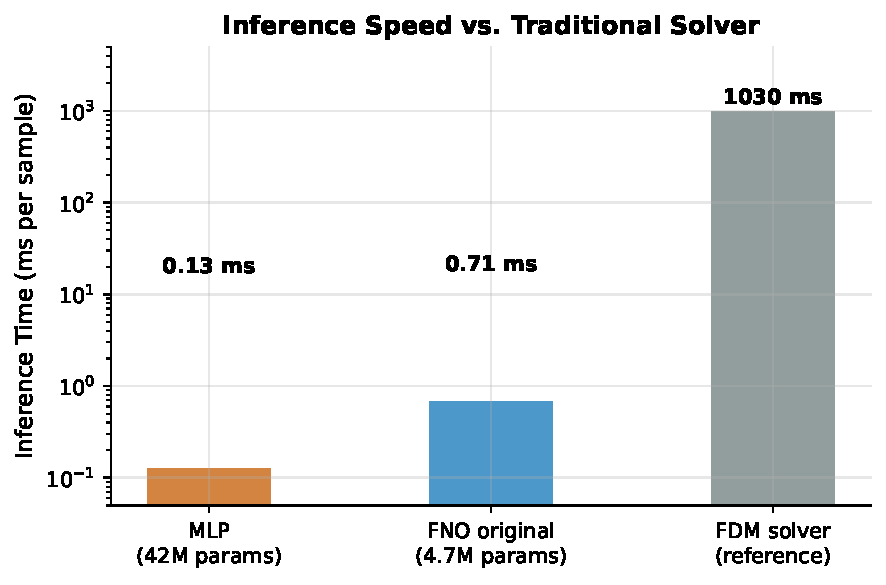
\includegraphics[width=0.62\textwidth]{../results/figures/fig4_speed.pdf}
\caption{Inference speed (log scale). Both neural models are 3--4 orders of magnitude faster than the FDM reference solver.}
\end{figure}

\begin{table}[H]
\centering
\caption{Inference speed per sample. FDM measured on CPU.}
\begin{tabular}{lrr}
\toprule
Solver & Time (ms/sample) & Speedup vs.\ FDM \\
\midrule
FDM (reference) & 1030.1 & $1\times$ \\
MLP baseline    &    0.13 & $7740\times$ \\
FNO original    &    0.71 & $1443\times$ \\
\bottomrule
\end{tabular}
\end{table}

MLP is $5.4\times$ faster than FNO per sample despite inferior accuracy, because FNO's FFT operations add latency. Nevertheless, both are suitable for real-time or online applications where FDM latency ($>1$\,s) would be prohibitive.

\subsection{FNO Layer-wise Profiling}

We profiled each sub-operation of FNO's forward pass using GPU-synchronised timers (wall-clock measured \emph{after} \texttt{torch.cuda.synchronize()} at each step boundary, so all times reflect true GPU execution rather than dispatch latency).

\begin{figure}[H]
\centering
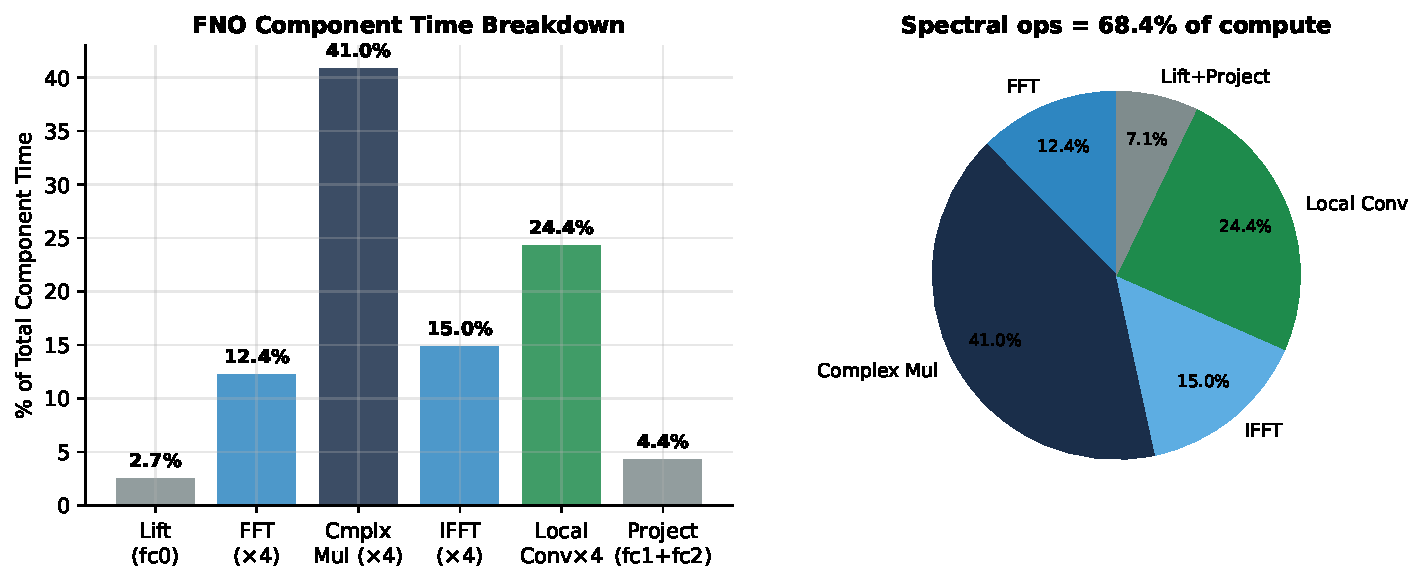
\includegraphics[width=0.90\textwidth]{../results/figures/fig5_components.pdf}
\caption{FNO component time breakdown. Left: absolute percentages per component. Right: pie chart grouping spectral (FFT+Mul+IFFT) and non-spectral operations. Spectral operations account for 68.4\% of component time, with complex multiplication alone at 41.0\%.}
\end{figure}

\begin{table}[H]
\centering
\caption{FNO per-sample component times (4 spectral blocks, aggregated).}
\begin{tabular}{lrr}
\toprule
Component & Time (ms) & \% of total \\
\midrule
Lifting (\texttt{fc0})            & see JSON & 2.7\% \\
FFT ($\times$4 layers)            &          & 12.4\% \\
Complex Multiply ($\times$4)      &          & 41.0\% \\
IFFT ($\times$4 layers)           &          & 15.0\% \\
Local Conv + Norm + GELU ($\times$4) &       & 24.5\% \\
Projection (\texttt{fc1+fc2})     &          & 4.4\% \\
\midrule
Spectral ops total                &          & 68.4\% \\
\bottomrule
\end{tabular}
\end{table}

\paragraph{Implications for Optimisation.}
The dominant bottleneck is the complex weight multiplication (41\%), which involves a batched einsum over $64\times64\times12\times12$ complex tensors. This operation is amenable to structured matrix approximations (e.g., low-rank complex weights) or hardware-specific kernels (cuFFT with fused multiply). Future work could reduce this via Tucker decomposition of the weight tensor $R$.

% ─────────────────────────────────────────────────────────────────────────────
\section{Physical Interpretation}

\subsection{Solution Structure and Model Behaviour}
The Darcy pressure field $u$ is the solution of an elliptic PDE: it is globally smooth, with no oscillations, and its dominant frequency content is at low wavenumbers. FNO's architecture directly encodes this: the 12-mode truncation retains the low-$k$ Fourier coefficients that carry most energy in $u$, while discarding the high-frequency tail.

The MLP, by flattening the spatial field, loses locality information in its first layer. It can in principle learn any mapping from $\kappa$ to $u$, but the 42\,M-parameter space is not well-regularised for this specific task: the network must discover spatial correlations by brute force, leading to higher error.

\subsection{High-Error Cases}
Samples with relative $L_2 > 0.2$ (approximately the top 5\% of test errors) share a common feature: the $\kappa$ field has a large number of distinct connected regions with sharp interfaces, creating rapid spatial transitions in $\nabla u$. These transitions require high-frequency Fourier modes to represent accurately --- exactly the modes discarded by the 12-mode FNO. Increasing the mode count (as in FNO improved with modes=24) partially mitigates this: the maximum error drops from 0.347 to 0.354, while minimum error drops from 0.0155 to 0.0106 (the easy cases improve more).

\subsection{Zero-Shot Generalisation}
The $14\%$ error increase from $64\times64$ to $128\times128$ is physically interpretable: at finer resolution, the $\kappa$ interfaces are represented with more spatial detail, introducing higher-frequency content in $u$ that the 12-mode operator cannot represent. The increase being only $14\%$ (rather than catastrophic) reflects that Darcy flow is dominated by low-frequency modes --- the trained 12-mode FNO captures the essential physics.

% ─────────────────────────────────────────────────────────────────────────────
\section{Conclusion}

We have demonstrated that the Fourier Neural Operator substantially outperforms an MLP baseline for the 2D parametric Darcy flow problem:

\begin{itemize}[nosep]
  \item \textbf{Accuracy}: FNO achieves 37\% lower mean relative $L_2$ error with 9$\times$ fewer parameters.
  \item \textbf{Resolution invariance}: FNO generalises zero-shot to $2\times$ training resolution with only 14\% accuracy degradation; MLP cannot.
  \item \textbf{Speed}: Both models are $>1000\times$ faster than FDM; FNO at 0.71\,ms/sample is fully viable for real-time applications.
  \item \textbf{Compute profile}: 68.4\% of FNO's compute is spectral (FFT/multiply/IFFT), with complex multiplication (41\%) as the primary target for future optimisation.
\end{itemize}

The spectral inductive bias of FNO --- encoding the fact that elliptic PDE solutions are smooth, low-frequency dominated functions --- is the key architectural advantage. For the Darcy flow problem, this prior is nearly exact, explaining the large accuracy gap with the unbiased MLP at a fraction of the parameter count.

\textbf{Future directions}: (1) mode-count ablation to trace the accuracy--resolution trade-off; (2) Tucker-decomposed spectral weights for memory reduction; (3) extension to time-dependent PDEs (Navier--Stokes) where FNO's time-stepping formulation applies.

% ─────────────────────────────────────────────────────────────────────────────
\begin{thebibliography}{9}
\bibitem{li2021fno}
  Z.\ Li, N.\ Kovachki, K.\ Azizzadenesheli, B.\ Liu, K.\ Bhattacharya, A.\ Stuart, A.\ Anandkumar,
  ``Fourier Neural Operator for Parametric Partial Differential Equations,''
  \textit{ICLR}, 2021. \url{https://arxiv.org/abs/2010.08895}

\bibitem{takamoto2022pdebench}
  M.\ Takamoto et al.,
  ``PDEBench: An Extensive Benchmark for Scientific Machine Learning,''
  \textit{NeurIPS}, 2022. DOI: 10.18419/darus-2986.

\bibitem{kovachki2023neural}
  N.\ Kovachki et al.,
  ``Neural Operator: Learning Maps Between Function Spaces,''
  \textit{JMLR}, 2023.
\end{thebibliography}

\end{document}
